% 刚体转动数值模拟

\pentry{刚体运动方程(四元数)\upref{RBEMQt}}

这里给出使用 4 阶龙格库塔法模拟刚体绕固定点转动的 Matlab 代码. 程序中给出的默认参数用于模拟一个初始静止的长方体受到一个 $(1,1,1)$ 方向的大小为 $0.05$ 的恒力矩时的加速转动.

运行结果见\link{互动演示}{http://wuli.wiki/apps/rigBdRot.html}, 截图如\autoref{RBRNum_fig1}

\begin{figure}[ht]
\centering
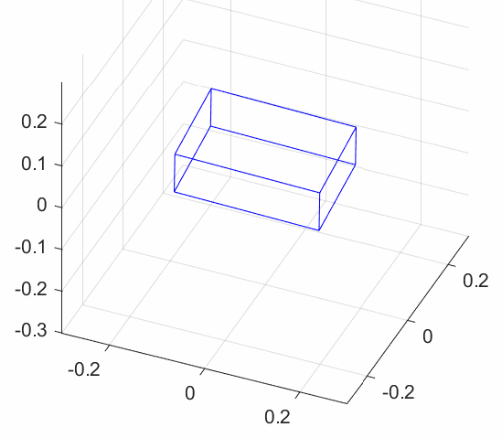
\includegraphics[width=8cm]{./figures/RBRNum1.png}
\caption{动画截图} \label{RBRNum_fig1}
\end{figure}.
\Code{rigBdRot}
